% ============================================================
%  يُترجَم بـ XeLaTeX  (في Overleaf: Menu → Compiler → XeLaTeX)
%  الخط: Amiri (متوفر في Overleaf، أو حمّله من github.com/aliftype/amiri)
% ============================================================
\documentclass[12pt,a4paper]{article}
\usepackage[a4paper,margin=1.7cm,top=2.3cm,bottom=2.9cm,headheight=15pt,footskip=1.5cm]{geometry}
\usepackage{amsmath,amssymb}
\usepackage{icomma}
\usepackage[english,bidi=default,layout=lists]{babel}
\babelprovide[import,main]{arabic}
\babelfont{rm}[Scale=1.08]{Amiri}
\babelfont{sf}[Scale=1.08]{Amiri}
\usepackage[most]{tcolorbox}
\usepackage{tikz}
\usetikzlibrary{arrows.meta,calc,shadings}
\usepackage{array}
\usepackage{colortbl}
\usepackage{fancyhdr}
\usepackage{titlesec}
\usepackage{enumitem}
\usepackage{collcell}
\usepackage{needspace}
\usepackage{etoolbox}
\newcolumntype{C}{>{\collectcell\ar}c<{\endcollectcell}}
\pretocmd{\section}{\Needspace{15\baselineskip}}{}{}
\pretocmd{\subsection}{\Needspace{11\baselineskip}}{}{}

\definecolor{cDef}{HTML}{1F4E9C}
\definecolor{cThm}{HTML}{B3261E}
\definecolor{cRem}{HTML}{2E7D32}
\definecolor{cEx}{HTML}{C76B00}
\definecolor{cMeth}{HTML}{6A1B9A}
\definecolor{cSol}{HTML}{00695C}
\definecolor{cSec}{HTML}{1F3A68}

\titleformat{\section}{\Large\bfseries\color{cSec}}{\thesection.}{0.6em}{}[{\color{cSec!60}\titlerule[1pt]}]
\titleformat{\subsection}{\large\bfseries\color{cThm!85!black}}{\thesubsection.}{0.5em}{}
\titlespacing*{\section}{0pt}{14pt}{8pt}
\titlespacing*{\subsection}{0pt}{10pt}{5pt}
\setlength{\parindent}{0pt}
\setlength{\parskip}{4pt}
\setlist{itemsep=2pt,topsep=3pt}

\newtcolorbox{arbox}[3][]{enhanced,
  colback=#2!5,colframe=#2!80!black,arc=2mm,boxrule=0.8pt,
  left=6pt,right=6pt,top=8pt,bottom=5pt,
  fonttitle=\bfseries,coltitle=white,
  title={\foreignlanguage{arabic}{#3}},
  attach boxed title to top right={xshift=-5mm,yshift=-3mm},
  boxed title style={colback=#2!80!black,arc=1.5mm,boxrule=0pt},
  before upper={\selectlanguage{arabic}},
  before skip=8pt,after skip=8pt,breakable,#1}
\newenvironment{BOX}[2]{\begin{otherlanguage}{english}\begin{arbox}{#1}{#2}}{\end{arbox}\end{otherlanguage}}
\newenvironment{tarif}[1][تعريف]{\begin{BOX}{cDef}{#1}}{\end{BOX}}
\newenvironment{khassia}[1][خاصية]{\begin{BOX}{cThm}{#1}}{\end{BOX}}
\newenvironment{molahada}[1][ملاحظة]{\begin{BOX}{cRem}{#1}}{\end{BOX}}
\newenvironment{mithal}[1][مثال]{\begin{BOX}{cEx}{#1}}{\end{BOX}}
\newenvironment{tariqa}[1][طريقة]{\begin{BOX}{cMeth}{#1}}{\end{BOX}}

\newcounter{exo}
\newenvironment{tamrin}[1]{\stepcounter{exo}\begin{BOX}{cSec}{التمرين \theexo: #1}}{\end{BOX}}
\newenvironment{hal}{\Needspace{12\baselineskip}\begin{otherlanguage}{english}\begin{arbox}[breakable]{cSol}{حل التمرين \theexo}}{\end{arbox}\end{otherlanguage}}

\newenvironment{LTR}{\begin{otherlanguage}{english}}{\end{otherlanguage}}
\newcommand{\ar}[1]{\foreignlanguage{arabic}{#1}}

\renewcommand{\dots}{\mathinner{\ldotp\ldotp\ldotp}}
\renewcommand{\ldots}{\mathinner{\ldotp\ldotp\ldotp}}
\renewcommand{\cdots}{\mathinner{\cdotp\cdotp\cdotp}}
\newcommand{\N}{\mathbb{N}}
\newcommand{\Z}{\mathbb{Z}}
\newcommand{\D}{\mathbb{D}}
\newcommand{\Q}{\mathbb{Q}}
\newcommand{\R}{\mathbb{R}}
\newcommand{\pgcd}{\operatorname{PGCD}}
\newcommand{\ppcm}{\operatorname{PPCM}}

% \NLseg{a}{b}{[}{]} ; \NLright{a}{[} ; \NLleft{b}{]}  (interval on a number line)
\newcommand{\NLseg}[4]{\begin{LTR}\begin{tikzpicture}[baseline=-0.6ex]
 \draw[-{Stealth[length=2mm]},gray!70](0,0)--(3.4,0);
 \draw[line width=2pt,cThm!80!black](0.7,0)--(2.7,0);
 \node[cThm!80!black,font=\LARGE] at (0.7,0){$#3$};
 \node[cThm!80!black,font=\LARGE] at (2.7,0){$#4$};
 \node[below=3pt,font=\footnotesize] at (0.7,0){$#1$};
 \node[below=3pt,font=\footnotesize] at (2.7,0){$#2$};
\end{tikzpicture}\end{LTR}}
\newcommand{\NLright}[2]{\begin{LTR}\begin{tikzpicture}[baseline=-0.6ex]
 \draw[-{Stealth[length=2mm]},gray!70](0,0)--(3.4,0);
 \draw[line width=2pt,cThm!80!black](1.3,0)--(3.3,0);
 \node[cThm!80!black,font=\LARGE] at (1.3,0){$#2$};
 \node[below=3pt,font=\footnotesize] at (1.3,0){$#1$};
\end{tikzpicture}\end{LTR}}
\newcommand{\NLleft}[2]{\begin{LTR}\begin{tikzpicture}[baseline=-0.6ex]
 \draw[-{Stealth[length=2mm]},gray!70](0,0)--(3.4,0);
 \draw[line width=2pt,cThm!80!black](0.05,0)--(2.1,0);
 \node[cThm!80!black,font=\LARGE] at (2.1,0){$#2$};
 \node[below=3pt,font=\footnotesize] at (2.1,0){$#1$};
\end{tikzpicture}\end{LTR}}

% ---------- social-media icons (pure TikZ) ----------
\definecolor{cFB}{HTML}{1877F2}
\definecolor{cTG}{HTML}{229ED9}
\definecolor{cIG1}{HTML}{FEDA75}
\definecolor{cIG2}{HTML}{D62976}
\definecolor{cIG3}{HTML}{4F5BD5}
\newcommand{\fbicon}{\begin{LTR}\begin{tikzpicture}[baseline=-0.75ex,x=1em,y=1em]
 \fill[cFB] (0,0) circle (0.55);
 \node[white,inner sep=0,font=\usefont{TU}{lmss}{bx}{n}\small] at (0.04,-0.02) {f};
\end{tikzpicture}\end{LTR}}
\newcommand{\igicon}{\begin{LTR}
\begin{tikzpicture}[baseline=-0.75ex,x=1em,y=1em]
 \shade[lower left=cIG1,lower right=cIG2,upper left=cIG2,upper right=cIG3,rounded corners=0.28em] (-0.55,-0.55) rectangle (0.55,0.55);
 \draw[white,line width=0.09em,rounded corners=0.18em] (-0.36,-0.36) rectangle (0.36,0.36);
 \draw[white,line width=0.09em] (0,0) circle (0.17);
 \fill[white] (0.22,0.22) circle (0.05);
\end{tikzpicture}\end{LTR}}
\newcommand{\tgicon}{\begin{LTR}
\begin{tikzpicture}[baseline=-0.75ex,x=1em,y=1em]
 \fill[cTG] (0,0) circle (0.55);
 \fill[white] (-0.33,0.0) -- (0.32,0.27) -- (0.2,-0.3) -- (0.0,-0.15) -- (-0.08,-0.28) -- (-0.08,-0.08) -- cycle;
 \fill[cTG!70!black] (-0.08,-0.08) -- (0.25,0.2) -- (0.0,-0.15) -- (-0.08,-0.28) -- cycle;
\end{tikzpicture}\end{LTR}}
% page number: black box, white two-digit number, at the right of the social row
\newcommand{\PageBox}{\begin{LTR}\tikz[baseline=(p.base)]\node[fill=black,text=white,inner sep=2.5pt,minimum width=1.6em,minimum height=1.3em,font=\usefont{TU}{lmss}{bx}{n}\small](p){\ifnum\value{page}<10 0\fi\arabic{page}};\end{LTR}}
% visual left-to-right order: Telegram | Instagram | Facebook | page box
\newcommand{\SocialRow}{\begin{otherlanguage}{english}%
 \ar{\textbf{الأستاذ سوايسية هشام للرياضيات}}\ \tgicon\hfill
 \textbf{prof\_hicham\_math}\ \igicon\hfill
 \ar{\textbf{الأستاذ سوايسية هشام للرياضيات}}\ \fbicon\hspace{2.2em}\PageBox\end{otherlanguage}}

\pagestyle{fancy}
\fancyhf{}
\renewcommand{\headrulewidth}{0.6pt}
\renewcommand{\footrulewidth}{0.4pt}
% \SetHeader{right head: document title}{left head: level -- stream}
\newcommand{\SetHeader}[2]{%
 \fancyhead[C]{\parbox{\textwidth}{\ar{#1\hfill #2}}}%
 \fancyfoot[C]{\parbox{\textwidth}{\small\SocialRow}}}
\usepackage{tkz-tab}
\usepackage{multicol}
% variation / sign table (LTR)
\newenvironment{TAB}{\par\begin{center}\begin{LTR}\begin{tikzpicture}[scale=0.95,every node/.style={font=\small}]}{\end{tikzpicture}\end{LTR}\end{center}}
% grid + axes, clipped: \begin{GR}{xmin}{xmax}{ymin}{ymax}{unit cm}
\newenvironment{GR}[5]{\par\begin{center}\begin{LTR}\begin{tikzpicture}[x=#5cm,y=#5cm,font=\footnotesize]
 \draw[gray!25,very thin] (#1,#3) grid (#2,#4);
 \draw[-{Stealth[length=2mm]}] (#1,0)--(#2+0.3,0) node[below left]{$x$};
 \draw[-{Stealth[length=2mm]}] (0,#3)--(0,#4+0.3) node[below left]{$y$};
 \node[below left] at (0,0){$O$};
 \begin{scope}\clip (#1,#3) rectangle (#2,#4);}
{\end{scope}\end{tikzpicture}\end{LTR}\end{center}}
\newcommand{\Ticks}[2]{\foreach \t in {#1} \node[below,font=\scriptsize] at (\t,0){$\t$}; \foreach \t in {#2} \node[left,font=\scriptsize] at (0,\t){$\t$};}
\newcommand{\bx}[1]{\ensuremath{\colorbox{cDef!12}{$\displaystyle #1$}}}
\newcommand{\TwoCol}[4]{\par\begin{LTR}\noindent\begin{minipage}[t]{#1\textwidth}\selectlanguage{arabic}#2\end{minipage}\hfill\begin{minipage}[t]{#3\textwidth}\selectlanguage{arabic}#4\end{minipage}\end{LTR}\par}
\newcommand{\RL}[4]{\TwoCol{#3}{#4}{#1}{#2}}  % \RL{w1}{right content}{w2}{left content}
\newcommand{\ok}{$\textcolor{cRem}{\checkmark}$}
\newcommand{\limn}{\displaystyle\lim_{n\to+\infty}}
% sub-questions, each on its own line
\newenvironment{sq}{\begin{itemize}[leftmargin=2.4em,itemsep=3pt]}{\end{itemize}}
\newcommand{\qa}{\item[(أ)]}\newcommand{\qb}{\item[(ب)]}\newcommand{\qc}{\item[(جـ)]}\newcommand{\qd}{\item[(د)]}\newcommand{\qe}{\item[(هـ)]}
\newcommand{\pa}{\par\smallskip\textbf{(أ)} }\newcommand{\pb}{\par\smallskip\textbf{(ب)} }\newcommand{\pc}{\par\smallskip\textbf{(جـ)} }\newcommand{\pd}{\par\smallskip\textbf{(د)} }\newcommand{\pe}{\par\smallskip\textbf{(هـ)} }
\newcommand{\QQ}[1]{\par\smallskip\textbf{#1.} }
\newenvironment{tmr}{\stepcounter{exo}\begin{BOX}{cSec}{تمرين محلول \theexo}}{\end{BOX}}
\newcommand{\ABC}[3]{\\[2pt]\begin{tabular}{p{0.28\textwidth}p{0.28\textwidth}p{0.28\textwidth}}(جـ) \ #3 & (ب) \ #2 & (أ) \ #1\end{tabular}}
\pretocmd{\section}{\Needspace{24\baselineskip}}{}{}
\newtcbox{\bxtbox}{on line,colback=cDef!12,colframe=cDef!12,boxrule=0pt,arc=1pt,boxsep=0pt,left=2pt,right=2pt,top=1pt,bottom=1pt}
\newcommand{\bxt}[1]{\foreignlanguage{english}{\bxtbox{\ar{#1}}}}
\SetHeader{\small\bfseries\color{cSec}تمارين تجريبية: الاحتمالات}{\small\color{cSec}السنة الثالثة ثانوي -- الشعب العلمية}
\begin{document}
\begin{LTR}
\begin{tcolorbox}[enhanced,colback=cSec,colframe=cSec,arc=3mm,halign=center,boxrule=0pt,top=12pt,bottom=12pt,before upper={\selectlanguage{arabic}}]
{\color{white}\fontsize{26}{32}\selectfont\bfseries تمارين تجريبية في الاحتمالات}\\[8pt]
{\color{white}\large تمارين متدرجة مع الحلول المفصلة خطوة بخطوة}\\[5pt]
{\color{white}\large السنة الثالثة ثانوي -- الشعب العلمية}
\end{tcolorbox}
\end{LTR}
% ================= تمارين تدريبية: الاحتمالات =================
\section{العدّ}

\begin{tamrin}{القوائم والترتيبات: الرمز السري}
رمز سري لهاتف يتكون من 4 أرقام مأخوذة من بين الأرقام $0,1,2,\ldots,9$ (مثلًا: $0725$ أو $3311$).
\QQ{1} ما عدد الرموز السرية الممكنة؟
\QQ{2} ما عدد الرموز المكونة من 4 أرقام مختلفة مثنى مثنى؟
\QQ{3} ما عدد الرموز المكونة من 4 أرقام مختلفة مثنى مثنى ولا تبدأ بالرقم $0$؟
\QQ{4} ما عدد الرموز التي تحتوي على الرقم $0$ مرة واحدة على الأقل؟
\end{tamrin}
\begin{hal}
\QQ{1} الرمز هو قائمة مرتبة من 4 عناصر من مجموعة بها 10 عناصر، والتكرار مسموح (يمكن أن يتكرر الرقم).
لكل خانة من الخانات الأربع 10 اختيارات، إذن حسب مبدأ الضرب:
\[10\times10\times10\times10=10^4=\bx{10000}\ \text{رمز}.\]
\QQ{2} الأرقام مختلفة مثنى مثنى والترتيب مهم (الرمز $1234$ يختلف عن $4321$)، فهو ترتيبة لـ 4 عناصر من بين 10 بدون تكرار:
\[A_{10}^4=10\times9\times8\times7=\bx{5040}.\]
\QQ{3} الخانة الأولى لا تقبل $0$: لها 9 اختيارات. بعد اختيارها يبقى 9 أرقام (منها $0$) لملء الخانات الثلاث الباقية بأرقام مختلفة، أي $A_9^3=9\times8\times7=504$ إمكانية. إذن:
\[9\times A_9^3=9\times504=\bx{4536}.\]
طريقة ثانية: من الـ $5040$ رمزًا ذات الأرقام المختلفة نطرح التي تبدأ بـ $0$ وعددها $A_9^3=504$: $5040-504=4536$ \ok.
\QQ{4} نستعمل الحدث العكسي: «لا يحتوي الرمز على $0$» معناه أن كل خانة تأخذ رقمًا من بين 9 أرقام، وعددها $9^4=6561$. إذن عدد الرموز التي تحتوي $0$ على الأقل مرة:
\[10^4-9^4=10000-6561=\bx{3439}.\]
\end{hal}

\begin{tamrin}{التوفيقات: تشكيل لجنة}
قسم به 20 تلميذًا: 12 بنتًا و8 أولاد. نريد تشكيل لجنة من 3 تلاميذ.
\QQ{1} ما عدد اللجان الممكنة؟
\QQ{2} ما عدد اللجان المكونة من بنتين وولد واحد بالضبط؟
\QQ{3} ما عدد اللجان التي تضم ولدًا واحدًا على الأقل؟
\QQ{4} علي تلميذ من هذا القسم. ما عدد اللجان التي يكون علي عضوًا فيها؟
\QQ{5} نريد الآن اختيار رئيس ونائب رئيس وكاتب (3 مهام مختلفة لثلاثة تلاميذ مختلفين). ما عدد الإمكانيات؟
\end{tamrin}
\begin{hal}
\QQ{1} اللجنة مجموعة جزئية من 3 تلاميذ: الترتيب غير مهم ولا تكرار، فهي توفيقة:
\[C_{20}^3=\frac{20\times19\times18}{3\times2\times1}=\bx{1140}.\]
\QQ{2} نختار بنتين من 12 ثم ولدًا من 8 (مبدأ الضرب):
\[C_{12}^2\times C_8^1=66\times8=\bx{528}.\]
\QQ{3} الحدث العكسي لـ «ولد واحد على الأقل» هو «لا يوجد أي ولد» أي اللجنة كلها بنات، وعددها $C_{12}^3=220$. إذن:
\[C_{20}^3-C_{12}^3=1140-220=\bx{920}.\]
\QQ{4} علي داخل اللجنة، فيبقى اختيار عضوين آخرين من بين التلاميذ الـ 19 الآخرين:
\[C_{19}^2=\frac{19\times18}{2}=\bx{171}.\]
\QQ{5} هنا الترتيب مهم (رئيس، نائب، كاتب) ولا تكرار، فهي ترتيبة:
\[A_{20}^3=20\times19\times18=\bx{6840}.\]
\begin{molahada}
لاحظ أن $A_{20}^3=3!\times C_{20}^3=6\times1140=6840$: كل لجنة من 3 أشخاص تعطي $3!=6$ طرق لتوزيع المهام.
\end{molahada}
\end{hal}

\begin{tamrin}{التبديلات: ترتيب كتب على رف}
نرتب على رف 5 كتب رياضيات مختلفة و3 كتب فيزياء مختلفة.
\QQ{1} ما عدد الترتيبات الممكنة؟
\QQ{2} ما عدد الترتيبات التي تكون فيها كتب الرياضيات متجاورة؟
\QQ{3} ما عدد الترتيبات التي تكون فيها كتب كل مادة متجاورة؟
\QQ{4} ما عدد الترتيبات التي لا يتجاور فيها أي كتابي فيزياء؟
\end{tamrin}
\begin{hal}
\QQ{1} نرتب 8 كتب مختلفة في 8 أماكن: هذا تبديلة لـ 8 عناصر:
\[8!=\bx{40320}.\]
\QQ{2} نعتبر كتب الرياضيات الخمسة «كتلة» واحدة. فيصبح لدينا $1+3=4$ عناصر نرتبها بـ $4!=24$ طريقة، وداخل الكتلة نرتب الكتب الخمسة بـ $5!=120$ طريقة. إذن:
\[4!\times5!=24\times120=\bx{2880}.\]
\QQ{3} لدينا كتلتان (رياضيات، فيزياء) ترتبان بـ $2!=2$ طريقة، وداخل كل كتلة: $5!$ و$3!$. إذن:
\[2!\times5!\times3!=2\times120\times6=\bx{1440}.\]
\QQ{4} نرتب أولًا كتب الرياضيات: $5!=120$ طريقة. فتنشأ 6 فراغات (قبل الأول، بين كل كتابين، بعد الأخير):
\[\_\ M\ \_\ M\ \_\ M\ \_\ M\ \_\ M\ \_\]
لكي لا يتجاور كتابا فيزياء نضع كل كتاب فيزياء في فراغ مختلف: نختار 3 فراغات مرتبة من 6 (الكتب مختلفة)، أي $A_6^3=6\times5\times4=120$ طريقة. إذن:
\[5!\times A_6^3=120\times120=\bx{14400}.\]
\end{hal}

\section{السحب في آن واحد وعلى التوالي}

\begin{tamrin}{سحب في آن واحد}
يحتوي كيس على 9 كريات متماثلة لا نفرق بينها باللمس: 4 حمراء، 3 خضراء وكريتان بيضاوان. نسحب عشوائيًا وفي آن واحد 3 كريات.
\QQ{1} ما عدد الحالات الممكنة؟
\QQ{2} احسب احتمال كل حدث من الأحداث التالية:
\begin{sq}
\qa $A$: «الكريات الثلاث من نفس اللون».
\qb $B$: «الكريات الثلاث مختلفة الألوان مثنى مثنى».
\qc $C$: «سحب كرية بيضاء على الأقل».
\qd $D$: «سحب كريتين حمراوين بالضبط».
\end{sq}
\end{tamrin}
\begin{hal}
\QQ{1} السحب في آن واحد: الترتيب غير مهم ولا تكرار، فكل نتيجة توفيقة لـ 3 من 9:
\[\operatorname{card}\Omega=C_9^3=\frac{9\times8\times7}{6}=\bx{84}.\]
الكريات متماثلة لا نفرق بينها باللمس، إذن الحالات متساوية الاحتمال، ومنه $P(E)=\dfrac{\operatorname{card}E}{\operatorname{card}\Omega}$.
\QQ{2}
\pa نفس اللون: 3 حمراء ($C_4^3=4$) أو 3 خضراء ($C_3^3=1$)، ولا يمكن 3 بيضاء (يوجد 2 فقط):
\[P(A)=\frac{C_4^3+C_3^3}{84}=\frac{4+1}{84}=\bx{\frac{5}{84}}.\]
\pb ألوان مختلفة: كرية من كل لون:
\[P(B)=\frac{C_4^1\times C_3^1\times C_2^1}{84}=\frac{24}{84}=\bx{\frac{2}{7}}.\]
\pc الحدث العكسي $\overline{C}$: «لا توجد أي كرية بيضاء»، أي الكريات الثلاث من بين 7 كريات غير بيضاء:
\[P(\overline{C})=\frac{C_7^3}{84}=\frac{35}{84}=\frac{5}{12}\quad\text{إذن}\quad P(C)=1-\frac{5}{12}=\bx{\frac{7}{12}}.\]
\pd حمراوان من 4 وكرية ثالثة غير حمراء من 5:
\[P(D)=\frac{C_4^2\times C_5^1}{84}=\frac{6\times5}{84}=\frac{30}{84}=\bx{\frac{5}{14}}.\]
\end{hal}

\begin{tamrin}{سحب على التوالي بإرجاع وبدون إرجاع}
صندوق به 6 كريات متماثلة: ثلاث تحمل الرقم $1$، اثنتان تحملان الرقم $2$ وواحدة تحمل الرقم $0$.
\QQ{1} نسحب عشوائيًا كريتين على التوالي دون إرجاع.
\begin{sq}
\qa ما عدد الحالات الممكنة؟
\qb احسب احتمال الحدث $A$: «مجموع الرقمين يساوي 2».
\qc احسب احتمال الحدث $B$: «جداء الرقمين معدوم».
\qd احسب احتمال الحدث $C$: «الكرية الثانية تحمل الرقم 2».
\end{sq}
\QQ{2} نعيد التجربة لكن بالسحب على التوالي مع الإرجاع. احسب في هذه الحالة $P(A)$ و$P(B)$.
\end{tamrin}
\begin{hal}
\QQ{1}
\pa دون إرجاع والترتيب مهم: ترتيبة لـ 2 من 6:
\[\operatorname{card}\Omega=A_6^2=6\times5=\bx{30}.\]
\pb المجموع 2 يتحقق بثلاث طرق:
\begin{itemize}
\item $(1;1)$: الأولى من الثلاث التي تحمل $1$ والثانية من الاثنتين الباقيتين: $A_3^2=3\times2=6$.
\item $(2;0)$: $2\times1=2$. \quad $(0;2)$: $1\times2=2$.
\end{itemize}
\[P(A)=\frac{6+2+2}{30}=\frac{10}{30}=\bx{\frac13}.\]
\pc الجداء معدوم إذا وفقط إذا ظهرت الكرية $0$ في أحد السحبين: $(0;\ast)$ عددها $1\times5=5$ و$(\ast;0)$ عددها $5\times1=5$:
\[P(B)=\frac{5+5}{30}=\bx{\frac13}.\]
\pd الكرية الثانية تحمل $2$: إما الأولى تحمل $2$ أيضًا ($2\times1=2$ حالة)، أو الأولى لا تحمل $2$ ($4\times2=8$ حالات):
\[P(C)=\frac{2+8}{30}=\bx{\frac13}.\]
نلاحظ أن $P(C)=\dfrac26$ وهو نفس احتمال أن تحمل الكرية الأولى الرقم $2$.
\QQ{2} مع الإرجاع: لكل سحب 6 اختيارات، إذن $\operatorname{card}\Omega=6^2=36$ (قائمة بتكرار).
\begin{itemize}
\item $A$: $(1;1)$: $3\times3=9$، $(2;0)$: $2\times1=2$، $(0;2)$: $1\times2=2$، ومنه $P(A)=\dfrac{13}{36}$.
\item $\overline{B}$: «الرقمان غير معدومين»: $5\times5=25$ حالة، ومنه $P(B)=1-\dfrac{25}{36}=\dfrac{11}{36}$.
\end{itemize}
\[\bx{P(A)=\frac{13}{36}}\qquad \bx{P(B)=\frac{11}{36}}\]
\end{hal}

\begin{tamrin}{مقارنة أنواع السحب الثلاثة}
كيس به 5 كريات متماثلة: 3 بيضاء و2 سوداء. نسحب كريتين وفق كل نمط من الأنماط التالية:
(I) في آن واحد، (II) على التوالي دون إرجاع، (III) على التوالي مع إرجاع.
\QQ{1} في كل نمط، احسب عدد الحالات الممكنة.
\QQ{2} في كل نمط، احسب احتمال الحدث $E$: «الكريتان من نفس اللون» واحتمال الحدث $F$: «الكريتان مختلفتا اللون».
\QQ{3} في النمطين (II) و(III)، احسب احتمال الحدث $G$: «الأولى بيضاء والثانية سوداء».
\QQ{4} ماذا تلاحظ؟
\end{tamrin}
\begin{hal}
\QQ{1}
\begin{itemize}
\item (I) توفيقة: $C_5^2=10$.
\item (II) ترتيبة: $A_5^2=5\times4=20$.
\item (III) قائمة بتكرار: $5^2=25$.
\end{itemize}
\QQ{2} في كل نمط: $F=\overline{E}$ إذن $P(F)=1-P(E)$.
\begin{itemize}
\item (I): $P(E)=\dfrac{C_3^2+C_2^2}{10}=\dfrac{3+1}{10}=\dfrac25$ \quad و\quad $P(F)=\dfrac{C_3^1\times C_2^1}{10}=\dfrac{6}{10}=\dfrac35$.
\item (II): $P(E)=\dfrac{A_3^2+A_2^2}{20}=\dfrac{6+2}{20}=\dfrac25$ \quad و\quad $P(F)=1-\dfrac25=\dfrac35$.
\item (III): $P(E)=\dfrac{3^2+2^2}{25}=\dfrac{13}{25}$ \quad و\quad $P(F)=1-\dfrac{13}{25}=\dfrac{12}{25}$.
\end{itemize}
\[\bx{P_{\rm I}(E)=P_{\rm II}(E)=\frac25}\qquad\bx{P_{\rm III}(E)=\frac{13}{25}}\]
\QQ{3} (II): $P(G)=\dfrac{3\times2}{20}=\bx{\dfrac{3}{10}}$\qquad (III): $P(G)=\dfrac{3\times2}{25}=\bx{\dfrac{6}{25}}$.
\QQ{4} السحب في آن واحد والسحب على التوالي دون إرجاع يعطيان نفس الاحتمالات للأحداث التي لا يهم فيها الترتيب، أما السحب مع الإرجاع فيعطي احتمالات مختلفة لأن الكرية المسحوبة يمكن أن تُسحب مرة ثانية.
\end{hal}

\section{قانون الاحتمال والمتغير العشوائي}

\begin{tamrin}{لعبة بنرد}
نرمي نردًا متوازنًا وجوهه مرقمة من 1 إلى 6. إذا ظهر الرقم 6 يربح اللاعب 10 نقاط، وإذا ظهر 4 أو 5 يربح نقطتين، وفي باقي الحالات يخسر 3 نقاط. ليكن $X$ المتغير العشوائي الذي يرفق بكل رمية ربح اللاعب (الخسارة ربح سالب).
\QQ{1} عيّن قيم $X$ ثم عرّف قانون احتماله.
\QQ{2} احسب الأمل الرياضياتي $E(X)$. هل اللعبة في صالح اللاعب؟
\QQ{3} احسب التباين $V(X)$ والانحراف المعياري $\sigma(X)$.
\QQ{4} احسب $P(X>0)$.
\end{tamrin}
\begin{hal}
\QQ{1} النرد متوازن: كل وجه احتماله $\dfrac16$. قيم $X$ هي $-3$، $2$، $10$:
\begin{itemize}
\item $P(X=-3)=P(\{1;2;3\})=\dfrac36=\dfrac12$.
\item $P(X=2)=P(\{4;5\})=\dfrac26=\dfrac13$.
\item $P(X=10)=P(\{6\})=\dfrac16$.
\end{itemize}
\begin{center}
\begin{tabular}{|C|c|c|c|C|}\hline
\rowcolor{cSec!12} $x_i$ & $-3$ & $2$ & $10$ & المجموع\\\hline
$P(X=x_i)$ & $\dfrac12$ & $\dfrac13$ & $\dfrac16$ & $1$\rule{0pt}{17pt}\\[6pt]\hline
\end{tabular}
\end{center}
\QQ{2}
\[E(X)=\sum x_iP(X=x_i)=(-3)\times\frac12+2\times\frac13+10\times\frac16=\frac{-9+4+10}{6}=\bx{\frac56}.\]
$E(X)>0$: إذن اللعبة \textbf{في صالح اللاعب} (يربح في المتوسط $\frac56$ نقطة في كل رمية).
\QQ{3} نحسب أولًا:
\[E(X^2)=(-3)^2\times\frac12+2^2\times\frac13+10^2\times\frac16=\frac{27+8+100}{6}=\frac{135}{6}=\frac{45}{2}.\]
\[V(X)=E(X^2)-\big(E(X)\big)^2=\frac{45}{2}-\frac{25}{36}=\frac{810-25}{36}=\bx{\frac{785}{36}}.\]
\[\sigma(X)=\sqrt{V(X)}=\frac{\sqrt{785}}{6}\approx\bx{4{,}67}.\]
\QQ{4} $P(X>0)=P(X=2)+P(X=10)=\dfrac13+\dfrac16=\bx{\dfrac12}$.
\end{hal}

\begin{tamrin}{عدد الكريات السوداء المسحوبة}
يحتوي صندوق على 4 كريات بيضاء و3 كريات سوداء، متماثلة لا نفرق بينها باللمس. نسحب عشوائيًا وفي آن واحد 3 كريات. ليكن $X$ المتغير العشوائي الذي يرفق بكل سحب عدد الكريات السوداء المسحوبة.
\QQ{1} عيّن قيم $X$ ثم عرّف قانون احتماله.
\QQ{2} احسب $E(X)$ و$V(X)$ و$\sigma(X)$.
\QQ{3} احسب $P(X\geqslant2)$ ثم $P(X^2-X=0)$.
\end{tamrin}
\begin{hal}
\QQ{1} $\operatorname{card}\Omega=C_7^3=35$. عدد الكريات السوداء بين 0 و3، إذن $X$ يأخذ القيم $0$، $1$، $2$، $3$.
\[P(X=0)=\frac{C_4^3}{35}=\frac{4}{35},\qquad P(X=1)=\frac{C_3^1C_4^2}{35}=\frac{3\times6}{35}=\frac{18}{35},\]
\[P(X=2)=\frac{C_3^2C_4^1}{35}=\frac{3\times4}{35}=\frac{12}{35},\qquad P(X=3)=\frac{C_3^3}{35}=\frac{1}{35}.\]
\begin{center}
\begin{tabular}{|C|c|c|c|c|C|}\hline
\rowcolor{cSec!12} $x_i$ & $0$ & $1$ & $2$ & $3$ & المجموع\\\hline
$P(X=x_i)$ & $\dfrac{4}{35}$ & $\dfrac{18}{35}$ & $\dfrac{12}{35}$ & $\dfrac{1}{35}$ & $1$\rule{0pt}{17pt}\\[6pt]\hline
\end{tabular}
\end{center}
التحقق: $4+18+12+1=35$ \ok.
\QQ{2}
\[E(X)=0\times\frac{4}{35}+1\times\frac{18}{35}+2\times\frac{12}{35}+3\times\frac{1}{35}=\frac{45}{35}=\bx{\frac97}.\]
\[E(X^2)=\frac{0+18+48+9}{35}=\frac{75}{35}=\frac{15}{7},\qquad V(X)=\frac{15}{7}-\frac{81}{49}=\frac{105-81}{49}=\bx{\frac{24}{49}}.\]
\[\sigma(X)=\sqrt{\frac{24}{49}}=\frac{2\sqrt6}{7}\approx\bx{0{,}70}.\]
\QQ{3}
\[P(X\geqslant2)=P(X=2)+P(X=3)=\frac{12+1}{35}=\bx{\frac{13}{35}}.\]
$X^2-X=0\iff X(X-1)=0\iff X=0$ أو $X=1$، إذن:
\[P(X^2-X=0)=\frac{4}{35}+\frac{18}{35}=\bx{\frac{22}{35}}.\]
\end{hal}

\begin{tamrin}{مجموع رقمين وتحويل تآلفي}
صندوق به 6 كريات متماثلة: كريتان تحملان الرقم $-1$، ثلاث كريات تحمل الرقم $0$ وكرية واحدة تحمل الرقم $2$. نسحب عشوائيًا وفي آن واحد كريتين. ليكن $X$ المتغير العشوائي الذي يرفق بكل سحب مجموع الرقمين المسجلين.
\QQ{1} بيّن أن قيم $X$ هي: $-2$، $-1$، $0$، $1$، $2$.
\QQ{2} عرّف قانون احتمال $X$.
\QQ{3} احسب $E(X)$ و$V(X)$ و$\sigma(X)$.
\QQ{4} احسب $P(|X|\leqslant1)$.
\QQ{5} نعتبر المتغير العشوائي $Y=2X+1$. استنتج $E(Y)$ و$V(Y)$.
\end{tamrin}
\begin{hal}
\QQ{1} الأزواج الممكنة (دون ترتيب) ومجاميعها:
\begin{itemize}
\item $\{-1;-1\}$: المجموع $-2$؛ \quad $\{-1;0\}$: $-1$؛ \quad $\{0;0\}$: $0$؛
\item $\{-1;2\}$: $1$؛ \quad $\{0;2\}$: $2$. (لا يمكن $\{2;2\}$ لأنه توجد كرية واحدة تحمل $2$).
\end{itemize}
إذن \bxt{قيم $X$ هي $-2$، $-1$، $0$، $1$، $2$}.
\QQ{2} $\operatorname{card}\Omega=C_6^2=15$.
\[P(X=-2)=\frac{C_2^2}{15}=\frac1{15},\quad P(X=-1)=\frac{C_2^1C_3^1}{15}=\frac6{15},\quad P(X=0)=\frac{C_3^2}{15}=\frac3{15},\]
\[P(X=1)=\frac{C_2^1C_1^1}{15}=\frac2{15},\quad P(X=2)=\frac{C_3^1C_1^1}{15}=\frac3{15}.\]
\begin{center}
\begin{tabular}{|C|c|c|c|c|c|C|}\hline
\rowcolor{cSec!12} $x_i$ & $-2$ & $-1$ & $0$ & $1$ & $2$ & المجموع\\\hline
$P(X=x_i)$ & $\dfrac{1}{15}$ & $\dfrac{6}{15}$ & $\dfrac{3}{15}$ & $\dfrac{2}{15}$ & $\dfrac{3}{15}$ & $1$\rule{0pt}{17pt}\\[6pt]\hline
\end{tabular}
\end{center}
\QQ{3}
\[E(X)=\frac{(-2)(1)+(-1)(6)+0(3)+1(2)+2(3)}{15}=\frac{-2-6+0+2+6}{15}=\bx{0}.\]
\[E(X^2)=\frac{4(1)+1(6)+0+1(2)+4(3)}{15}=\frac{24}{15}=\frac85,\quad V(X)=\frac85-0^2=\bx{\frac85}.\]
\[\sigma(X)=\sqrt{\frac85}=\frac{2\sqrt{10}}{5}\approx\bx{1{,}26}.\]
\QQ{4} $|X|\leqslant1\iff X\in\{-1;0;1\}$:
\[P(|X|\leqslant1)=\frac{6+3+2}{15}=\bx{\frac{11}{15}}.\]
\QQ{5} من خواص الأمل والتباين: $E(aX+b)=aE(X)+b$ و$V(aX+b)=a^2V(X)$:
\[E(Y)=2\times0+1=\bx{1},\qquad V(Y)=2^2\times\frac85=\bx{\frac{32}{5}}.\]
\end{hal}

\section{الاحتمال الشرطي وشجرة الاحتمالات}

\begin{tamrin}{جدول بمدخلين والاحتمال الشرطي}
في ثانوية بها 200 تلميذ في السنة الثالثة: 120 بنتًا و80 ولدًا. من بين البنات 90 يدرسن في شعبة علمية، ومن بين الأولاد 50 يدرسون في شعبة علمية. نختار تلميذًا عشوائيًا. نسمي $F$: «التلميذ بنت» و$S$: «التلميذ في شعبة علمية».
\QQ{1} أكمل الجدول بمدخلين التالي:
\begin{center}
\begin{tabular}{|C|C|C|C|}\hline
\rowcolor{cSec!12} & $S$ & $\overline{S}$ & المجموع\\\hline
$F$ & $90$ & $\ldots$ & $120$\\\hline
$\overline{F}$ & $50$ & $\ldots$ & $\ldots$\\\hline
المجموع & $\ldots$ & $\ldots$ & $200$\\\hline
\end{tabular}
\end{center}
\QQ{2} احسب $P(F)$، $P(S)$ و$P(F\cap S)$.
\QQ{3} احسب $P_F(S)$ ثم $P_S(F)$، وفسّر كل نتيجة.
\end{tamrin}
\begin{hal}
\QQ{1} $120-90=30$، $80-50=30$، $90+50=140$، $30+30=60$:
\begin{center}
\begin{tabular}{|C|C|C|C|}\hline
\rowcolor{cSec!12} & $S$ & $\overline{S}$ & المجموع\\\hline
$F$ & $90$ & $30$ & $120$\\\hline
$\overline{F}$ & $50$ & $30$ & $80$\\\hline
المجموع & $140$ & $60$ & $200$\\\hline
\end{tabular}
\end{center}
\QQ{2} الاختيار عشوائي (تساوي الاحتمال):
\[P(F)=\frac{120}{200}=\bx{\frac35},\qquad P(S)=\frac{140}{200}=\bx{\frac{7}{10}},\qquad P(F\cap S)=\frac{90}{200}=\bx{\frac{9}{20}}.\]
\QQ{3}
\[P_F(S)=\frac{P(F\cap S)}{P(F)}=\frac{9/20}{3/5}=\bx{\frac34}\]
أي: إذا علمنا أن التلميذ المختار بنت، فاحتمال أن تكون في شعبة علمية هو $\frac34$ (وهو $\frac{90}{120}$: نقتصر على سطر البنات).
\[P_S(F)=\frac{P(F\cap S)}{P(S)}=\frac{9/20}{7/10}=\bx{\frac{9}{14}}\]
أي: إذا علمنا أن التلميذ في شعبة علمية، فاحتمال أن يكون بنتًا هو $\frac{9}{14}$ (وهو $\frac{90}{140}$: نقتصر على عمود $S$).
\end{hal}

\begin{tamrin}{ثلاث آلات: الاحتمالات الكلية والسؤال العكسي}
مصنع ينتج قطعًا بثلاث آلات: الآلة $M_1$ تنتج $50\%$ من الإنتاج، و$M_2$ تنتج $30\%$، و$M_3$ تنتج الباقي. نسبة القطع المعيبة هي $2\%$ لإنتاج $M_1$، و$3\%$ لإنتاج $M_2$، و$5\%$ لإنتاج $M_3$. نختار قطعة عشوائيًا من الإنتاج الكلي. نسمي $D$: «القطعة معيبة» و$M_i$: «القطعة من إنتاج الآلة $M_i$».
\QQ{1} مثّل الوضعية بشجرة احتمالات.
\QQ{2} احسب $P(M_1\cap D)$.
\QQ{3} بيّن أن $P(D)=0.029$.
\QQ{4} القطعة المختارة معيبة. ما احتمال أن تكون من إنتاج الآلة $M_3$؟
\end{tamrin}
\begin{hal}
\QQ{1} $P(M_3)=1-0{,}5-0{,}3=0.2$. الاحتمالات الشرطية: $P_{M_1}(D)=0.02$، $P_{M_2}(D)=0.03$، $P_{M_3}(D)=0.05$.
\begin{center}\begin{LTR}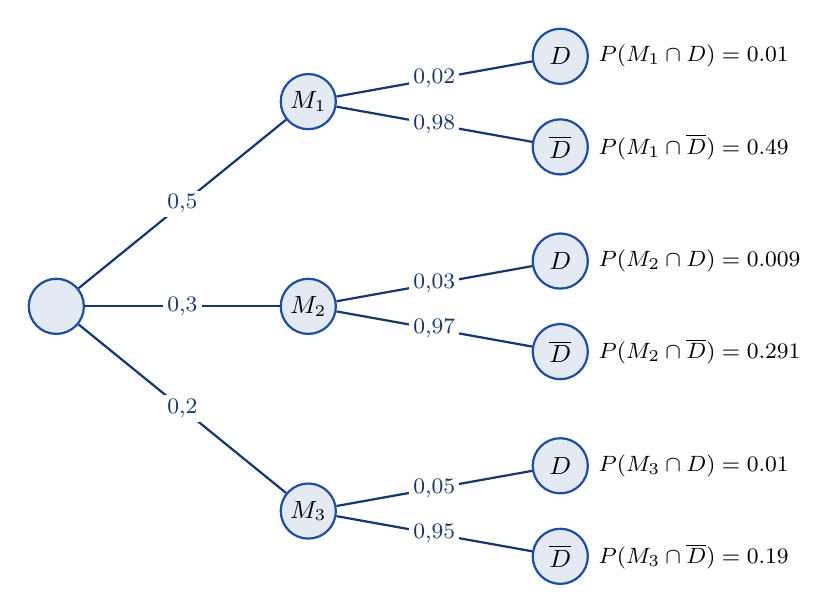
\begin{tikzpicture}[grow=right,level distance=3.2cm,
  level 1/.style={sibling distance=2.6cm}, level 2/.style={sibling distance=1.15cm},
  ev/.style={circle,draw=cDef,fill=cDef!12,thick,minimum size=7mm,inner sep=1pt,font=\small},
  edge from parent/.style={draw,thick,cDef!70!black},
  p/.style={midway,fill=white,inner sep=1.5pt,font=\footnotesize},
  lf/.style={label={[font=\footnotesize]right:#1}}]
\node[ev]{}
  child{node[ev]{$M_3$}
     child{node[ev,lf={$P(M_3\cap\overline{D})=0.19$}]{$\overline{D}$} edge from parent node[p]{$0{,}95$}}
     child{node[ev,lf={$P(M_3\cap D)=0.01$}]{$D$} edge from parent node[p]{$0{,}05$}}
     edge from parent node[p]{$0{,}2$}}
  child{node[ev]{$M_2$}
     child{node[ev,lf={$P(M_2\cap\overline{D})=0.291$}]{$\overline{D}$} edge from parent node[p]{$0{,}97$}}
     child{node[ev,lf={$P(M_2\cap D)=0.009$}]{$D$} edge from parent node[p]{$0{,}03$}}
     edge from parent node[p]{$0{,}3$}}
  child{node[ev]{$M_1$}
     child{node[ev,lf={$P(M_1\cap\overline{D})=0.49$}]{$\overline{D}$} edge from parent node[p]{$0{,}98$}}
     child{node[ev,lf={$P(M_1\cap D)=0.01$}]{$D$} edge from parent node[p]{$0{,}02$}}
     edge from parent node[p]{$0{,}5$}};
\end{tikzpicture}\end{LTR}\end{center}
\QQ{2} احتمال مسار = جداء الاحتمالات على أغصانه:
\[P(M_1\cap D)=P(M_1)\times P_{M_1}(D)=0.5\times0{,}02=\bx{0{,}01}.\]
\QQ{3} الأحداث $M_1$، $M_2$، $M_3$ تشكل تجزئة لـ $\Omega$ (غير متلائمة مثنى مثنى واتحادها $\Omega$)، إذن حسب دستور الاحتمالات الكلية:
\begin{align*}
P(D)&=P(M_1)P_{M_1}(D)+P(M_2)P_{M_2}(D)+P(M_3)P_{M_3}(D)\\
&=0.5\times0{,}02+0{,}3\times0{,}03+0{,}2\times0{,}05=0.01+0{,}009+0{,}01=\bx{0{,}029}.
\end{align*}
\QQ{4} المطلوب احتمال شرطي «عكسي» $P_D(M_3)$:
\[P_D(M_3)=\frac{P(M_3\cap D)}{P(D)}=\frac{0{,}01}{0{,}029}=\bx{\frac{10}{29}}\approx0{,}345.\]
\begin{molahada}
رغم أن $M_3$ تنتج $20\%$ فقط من القطع، فإن حوالي $34{,}5\%$ من القطع المعيبة تأتي منها، لأن نسبة العيب فيها هي الأكبر.
\end{molahada}
\end{hal}

\begin{tamrin}{صندوقان ونرد}
لدينا صندوقان: $U_1$ به 3 كريات بيضاء و2 حمراء، و$U_2$ به كرية بيضاء واحدة و3 حمراء. نرمي نردًا متوازنًا: إذا ظهر 1 أو 2 نسحب كرية من $U_1$، وإلا نسحب كرية من $U_2$. نسمي $U_1$: «السحب من الصندوق $U_1$» و$B$: «الكرية المسحوبة بيضاء».
\QQ{1} أنشئ شجرة الاحتمالات المناسبة.
\QQ{2} بيّن أن $P(B)=\dfrac{11}{30}$.
\QQ{3} علمًا أن الكرية المسحوبة بيضاء، ما احتمال أنها سُحبت من $U_1$؟
\QQ{4} علمًا أن الكرية المسحوبة حمراء، ما احتمال أنها سُحبت من $U_1$؟
\end{tamrin}
\begin{hal}
\QQ{1} $P(U_1)=\dfrac26=\dfrac13$ و$P(U_2)=\dfrac23$. في $U_1$: $P_{U_1}(B)=\dfrac35$؛ في $U_2$: $P_{U_2}(B)=\dfrac14$.
\begin{center}\begin{LTR}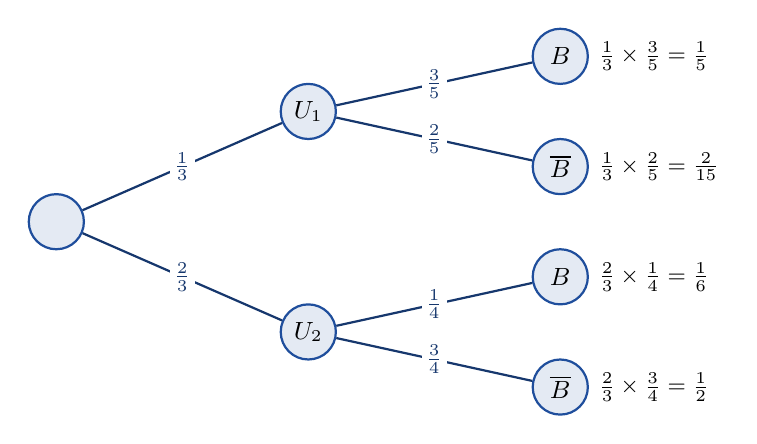
\begin{tikzpicture}[grow=right,level distance=3.2cm,
  level 1/.style={sibling distance=2.8cm}, level 2/.style={sibling distance=1.4cm},
  ev/.style={circle,draw=cDef,fill=cDef!12,thick,minimum size=7mm,inner sep=1pt,font=\small},
  edge from parent/.style={draw,thick,cDef!70!black},
  p/.style={midway,fill=white,inner sep=1.5pt,font=\footnotesize},
  lf/.style={label={[font=\footnotesize]right:#1}}]
\node[ev]{}
  child{node[ev]{$U_2$}
     child{node[ev,lf={$\frac23\times\frac34=\frac12$}]{$\overline{B}$} edge from parent node[p]{$\frac34$}}
     child{node[ev,lf={$\frac23\times\frac14=\frac16$}]{$B$} edge from parent node[p]{$\frac14$}}
     edge from parent node[p]{$\frac23$}}
  child{node[ev]{$U_1$}
     child{node[ev,lf={$\frac13\times\frac25=\frac{2}{15}$}]{$\overline{B}$} edge from parent node[p]{$\frac25$}}
     child{node[ev,lf={$\frac13\times\frac35=\frac15$}]{$B$} edge from parent node[p]{$\frac35$}}
     edge from parent node[p]{$\frac13$}};
\end{tikzpicture}\end{LTR}\end{center}
\QQ{2} $U_1$ و$U_2$ تجزئة لـ $\Omega$، حسب دستور الاحتمالات الكلية:
\[P(B)=P(U_1)P_{U_1}(B)+P(U_2)P_{U_2}(B)=\frac13\times\frac35+\frac23\times\frac14=\frac15+\frac16=\bx{\frac{11}{30}}.\]
\QQ{3}
\[P_B(U_1)=\frac{P(U_1\cap B)}{P(B)}=\frac{1/5}{11/30}=\frac15\times\frac{30}{11}=\bx{\frac{6}{11}}.\]
\QQ{4} $P(\overline{B})=1-\dfrac{11}{30}=\dfrac{19}{30}$، و$P(U_1\cap\overline{B})=\dfrac{2}{15}$، إذن:
\[P_{\overline{B}}(U_1)=\frac{2/15}{19/30}=\frac{2}{15}\times\frac{30}{19}=\bx{\frac{4}{19}}.\]
\end{hal}

\begin{tamrin}{سحب مع إضافة كرية من نفس اللون}
يحتوي صندوق على 3 كريات حمراء وكريتين خضراوين. نسحب كرية، نسجل لونها ثم نعيدها إلى الصندوق ونضيف معها كرية أخرى من نفس لونها، ثم نسحب كرية ثانية. نسمي $R_1$: «الكرية الأولى حمراء» و$R_2$: «الكرية الثانية حمراء».
\QQ{1} احسب $P_{R_1}(R_2)$ و$P_{\overline{R_1}}(R_2)$، ثم أنشئ شجرة الاحتمالات.
\QQ{2} احسب $P(R_2)$. قارنه بـ $P(R_1)$.
\QQ{3} علمًا أن الكرية الثانية حمراء، ما احتمال أن تكون الأولى حمراء أيضًا؟
\QQ{4} احسب احتمال الحدث $E$: «الكريتان من نفس اللون».
\end{tamrin}
\begin{hal}
\QQ{1} في البداية 5 كريات، إذن $P(R_1)=\dfrac35$ و$P(\overline{R_1})=\dfrac25$.
\begin{itemize}
\item إذا كانت الأولى حمراء: يصبح في الصندوق 4 حمراء و2 خضراء (6 كريات)، ومنه $P_{R_1}(R_2)=\dfrac46=\dfrac23$.
\item إذا كانت الأولى خضراء: يصبح 3 حمراء و3 خضراء، ومنه $P_{\overline{R_1}}(R_2)=\dfrac36=\dfrac12$.
\end{itemize}
\begin{center}\begin{LTR}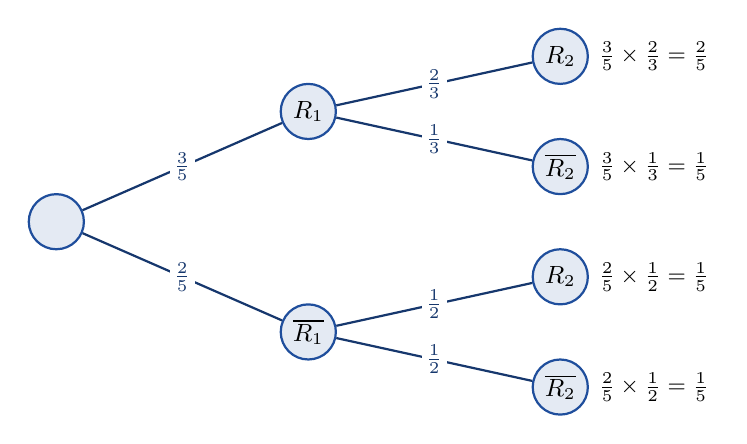
\begin{tikzpicture}[grow=right,level distance=3.2cm,
  level 1/.style={sibling distance=2.8cm}, level 2/.style={sibling distance=1.4cm},
  ev/.style={circle,draw=cDef,fill=cDef!12,thick,minimum size=7mm,inner sep=1pt,font=\small},
  edge from parent/.style={draw,thick,cDef!70!black},
  p/.style={midway,fill=white,inner sep=1.5pt,font=\footnotesize},
  lf/.style={label={[font=\footnotesize]right:#1}}]
\node[ev]{}
  child{node[ev]{$\overline{R_1}$}
     child{node[ev,lf={$\frac25\times\frac12=\frac15$}]{$\overline{R_2}$} edge from parent node[p]{$\frac12$}}
     child{node[ev,lf={$\frac25\times\frac12=\frac15$}]{$R_2$} edge from parent node[p]{$\frac12$}}
     edge from parent node[p]{$\frac25$}}
  child{node[ev]{$R_1$}
     child{node[ev,lf={$\frac35\times\frac13=\frac15$}]{$\overline{R_2}$} edge from parent node[p]{$\frac13$}}
     child{node[ev,lf={$\frac35\times\frac23=\frac25$}]{$R_2$} edge from parent node[p]{$\frac23$}}
     edge from parent node[p]{$\frac35$}};
\end{tikzpicture}\end{LTR}\end{center}
\QQ{2} حسب دستور الاحتمالات الكلية ($R_1$ و$\overline{R_1}$ تجزئة لـ $\Omega$):
\[P(R_2)=P(R_1)P_{R_1}(R_2)+P(\overline{R_1})P_{\overline{R_1}}(R_2)=\frac25+\frac15=\bx{\frac35}.\]
نلاحظ أن $P(R_2)=P(R_1)=\dfrac35$.
\QQ{3}
\[P_{R_2}(R_1)=\frac{P(R_1\cap R_2)}{P(R_2)}=\frac{2/5}{3/5}=\bx{\frac23}.\]
\QQ{4} $E=(R_1\cap R_2)\cup(\overline{R_1}\cap\overline{R_2})$ والحدثان غير متلائمين:
\[P(E)=\frac25+\frac15=\bx{\frac35}.\]
\end{hal}

\section{الاستقلالية}

\begin{tamrin}{حدثان مستقلان}
\QQ{1} $A$ و$B$ حدثان مستقلان من فضاء احتمالي حيث $P(A)=0.4$ و$P(B)=0.5$. احسب:
\begin{sq}
\qa $P(A\cap B)$ و$P(A\cup B)$.
\qb $P(\overline{A}\cap\overline{B})$ ثم تحقق أنه يساوي $P(\overline{A})\times P(\overline{B})$.
\qc $P(A\cap\overline{B})$.
\end{sq}
\QQ{2} نرمي نردًا متوازنًا مرة واحدة. نعتبر الأحداث: $A$: «ظهور رقم زوجي»، $B$: «ظهور رقم أصغر من أو يساوي 2»، $C$: «ظهور رقم أكبر من أو يساوي 4».
\begin{sq}
\qa هل الحدثان $A$ و$B$ مستقلان؟
\qb هل الحدثان $A$ و$C$ مستقلان؟
\end{sq}
\end{tamrin}
\begin{hal}
\QQ{1}
\pa بما أن $A$ و$B$ مستقلان: $P(A\cap B)=P(A)\times P(B)=0.4\times0{,}5=\bx{0{,}2}$.
\[P(A\cup B)=P(A)+P(B)-P(A\cap B)=0.4+0{,}5-0{,}2=\bx{0{,}7}.\]
\pb حسب قانون دي مورغان: $\overline{A}\cap\overline{B}=\overline{A\cup B}$، إذن:
\[P(\overline{A}\cap\overline{B})=1-P(A\cup B)=1-0{,}7=\bx{0{,}3}.\]
و$P(\overline{A})\times P(\overline{B})=0.6\times0{,}5=0.3$ \ok: الحدثان $\overline{A}$ و$\overline{B}$ مستقلان أيضًا.
\pc $A=(A\cap B)\cup(A\cap\overline{B})$ (اتحاد غير متلائم)، إذن:
\[P(A\cap\overline{B})=P(A)-P(A\cap B)=0.4-0{,}2=\bx{0{,}2}.\]
\QQ{2} $\Omega=\{1;2;3;4;5;6\}$ وتساوي الاحتمال. $A=\{2;4;6\}$، $B=\{1;2\}$، $C=\{4;5;6\}$.
\pa $A\cap B=\{2\}$، إذن $P(A\cap B)=\dfrac16$، و$P(A)\times P(B)=\dfrac12\times\dfrac13=\dfrac16$.

بما أن $P(A\cap B)=P(A)\times P(B)$ فإن \bxt{$A$ و$B$ مستقلان}.
\pb $A\cap C=\{4;6\}$، إذن $P(A\cap C)=\dfrac26=\dfrac13$، بينما $P(A)\times P(C)=\dfrac12\times\dfrac12=\dfrac14$.

بما أن $\dfrac13\neq\dfrac14$ فإن \bxt{$A$ و$C$ غير مستقلين}.
\end{hal}

\begin{tamrin}{دارة بثلاث مركبات مستقلة}
جهاز يحتوي على ثلاث مركبات $C_1$، $C_2$، $C_3$ تعمل باستقلالية عن بعضها. احتمال أن تعمل كل منها خلال سنة هو على الترتيب: $0{,}9$ ، $0{,}8$ ، $0{,}7$.
\QQ{1} احسب احتمال أن تعمل المركبات الثلاث (تركيب على التسلسل).
\QQ{2} احسب احتمال أن تتعطل مركبة واحدة على الأقل.
\QQ{3} احسب احتمال أن تعمل مركبة واحدة على الأقل (تركيب على التفرع).
\QQ{4} احسب احتمال أن تعمل مركبة واحدة فقط.
\QQ{5} في الجهاز، $C_1$ مركبة على التسلسل مع المجموعة ($C_2$ و$C_3$ على التفرع) كما في الشكل. يعمل الجهاز إذا مر التيار من $E$ إلى $S$. احسب احتمال أن يعمل الجهاز.
\begin{center}\begin{LTR}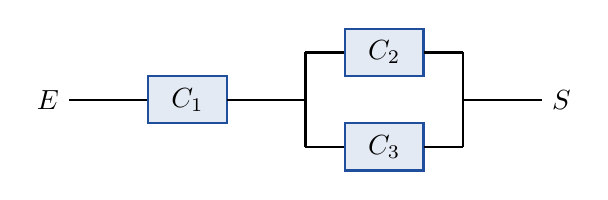
\begin{tikzpicture}[thick,b/.style={draw=cDef,fill=cDef!12,minimum width=10mm,minimum height=6mm}]
\node[left] at (0,0){$E$};
\draw (0,0)--(1,0); \node[b] (c1) at (1.5,0){$C_1$}; \draw (2,0)--(3,0);
\draw (3,0.6)--(3,-0.6); \draw (3,0.6)--(3.5,0.6); \draw (3,-0.6)--(3.5,-0.6);
\node[b] at (4,0.6){$C_2$}; \node[b] at (4,-0.6){$C_3$};
\draw (4.5,0.6)--(5,0.6); \draw (4.5,-0.6)--(5,-0.6); \draw (5,0.6)--(5,-0.6); \draw (5,0)--(6,0);
\node[right] at (6,0){$S$};
\end{tikzpicture}\end{LTR}\end{center}
\end{tamrin}
\begin{hal}
نسمي $F_i$: «المركبة $C_i$ تعمل». الأحداث $F_1$، $F_2$، $F_3$ مستقلة، فأضدادها مستقلة كذلك:
$P(\overline{F_1})=0.1$، $P(\overline{F_2})=0.2$، $P(\overline{F_3})=0.3$.
\QQ{1} بالاستقلالية:
\[P(F_1\cap F_2\cap F_3)=0.9\times0{,}8\times0{,}7=\bx{0{,}504}.\]
\QQ{2} «تتعطل مركبة على الأقل» هو عكس «تعمل الثلاث»:
\[1-0{,}504=\bx{0{,}496}.\]
\QQ{3} «تعمل مركبة على الأقل» هو عكس «تتعطل الثلاث»:
\[1-P(\overline{F_1}\cap\overline{F_2}\cap\overline{F_3})=1-0{,}1\times0{,}2\times0{,}3=1-0{,}006=\bx{0{,}994}.\]
\QQ{4} تعمل واحدة فقط: ثلاث حالات غير متلائمة:
\begin{align*}
P&=P(F_1\cap\overline{F_2}\cap\overline{F_3})+P(\overline{F_1}\cap F_2\cap\overline{F_3})+P(\overline{F_1}\cap\overline{F_2}\cap F_3)\\
&=0.9\times0{,}2\times0{,}3+0{,}1\times0{,}8\times0{,}3+0{,}1\times0{,}2\times0{,}7=0.054+0{,}024+0{,}014=\bx{0{,}092}.
\end{align*}
\QQ{5} يعمل الجهاز إذا عملت $C_1$ \textbf{و} عملت $C_2$ أو $C_3$ على الأقل. التفرع: $P(F_2\cup F_3)=1-0{,}2\times0{,}3=0.94$. نسمي $M$: «الجهاز يعمل». وبالاستقلالية:
\[P(M)=P(F_1)\times P(F_2\cup F_3)=0.9\times0{,}94=\bx{0{,}846}.\]
\end{hal}

\section{اختيار من متعدد وصحيح أم خطأ}

\begin{tamrin}{اختيار من متعدد}
اختر الإجابة الصحيحة الوحيدة في كل حالة مع التعليل.

\textbf{1.} عدد طرق جلوس 4 أشخاص على 4 كراسي مصفوفة هو:
\ABC{$16$}{$24$}{$4$}\par\medskip

\textbf{2.} العدد $C_7^3$ يساوي:
\ABC{$35$}{$210$}{$21$}\par\medskip

\textbf{3.} نسحب في آن واحد كريتين من كيس به 6 كريات. عدد الحالات الممكنة هو:
\ABC{$30$}{$36$}{$15$}\par\medskip

\textbf{4.} $A$ و$B$ مستقلان، $P(A)=0.3$ و$P(B)=0.6$. إذن $P(A\cup B)$ يساوي:
\ABC{$0{,}9$}{$0{,}72$}{$0{,}18$}\par\medskip

\textbf{5.} متغير عشوائي $X$ يأخذ القيم $-1$، $0$، $2$ باحتمالات $0{,}3$، $0{,}5$، $0{,}2$ على الترتيب. $E(X)$ يساوي:
\ABC{$0{,}1$}{$0{,}7$}{$0$}\par\medskip

\textbf{6.} $P(A)=0.5$، $P_A(B)=0.4$ و$P(\overline{A}\cap B)=0.1$. إذن $P(B)$ يساوي:
\ABC{$0{,}2$}{$0{,}5$}{$0{,}3$}
\end{tamrin}
\begin{hal}
\QQ{1} تبديلة لـ 4 عناصر: $4!=24$. الإجابة \bxt{(ب)}.
\QQ{2} $C_7^3=\dfrac{7\times6\times5}{3\times2\times1}=35$. الإجابة \bxt{(أ)}.
\QQ{3} توفيقة: $C_6^2=\dfrac{6\times5}{2}=15$. الإجابة \bxt{(جـ)}. ($30=A_6^2$ للسحب على التوالي دون إرجاع، و$36=6^2$ مع الإرجاع).
\QQ{4} $P(A\cap B)=0.3\times0{,}6=0.18$، ومنه $P(A\cup B)=0.3+0{,}6-0{,}18=0.72$. الإجابة \bxt{(ب)}.
\QQ{5} $E(X)=(-1)(0{,}3)+0(0{,}5)+2(0{,}2)=-0{,}3+0{,}4=0.1$. الإجابة \bxt{(أ)}.
\QQ{6} $P(A\cap B)=P(A)\times P_A(B)=0.5\times0{,}4=0.2$، وحسب الاحتمالات الكلية: $P(B)=P(A\cap B)+P(\overline{A}\cap B)=0.2+0{,}1=0.3$. الإجابة \bxt{(جـ)}.
\end{hal}

\begin{tamrin}{صحيح أم خطأ}
أجب بـ «صحيح» أو «خطأ» مع التعليل ($n$ و$p$ عددان طبيعيان، $0\leqslant p\leqslant n$).

\textbf{1.} $A_n^p=p!\times C_n^p$.\par
\textbf{2.} إذا كان $A$ و$B$ حدثين غير متلائمين واحتمال كل منهما غير معدوم، فإنهما مستقلان.\par
\textbf{3.} $C_n^p=C_n^{n-p}$.\par
\textbf{4.} إذا كان $V(X)=4$ فإن $V(3X+1)=37$.\par
\textbf{5.} عدد الكلمات المكونة من 3 حروف (لها معنى أو لا) من الحروف $a$، $b$، $c$، $d$ مع إمكانية التكرار هو $64$.\par
\textbf{6.} نرمي قطعة نقدية متوازنة 3 مرات. احتمال الحصول على الوجه مرتين بالضبط هو $\dfrac14$.
\end{tamrin}
\begin{hal}
\QQ{1} \bxt{صحيح}: $A_n^p=\dfrac{n!}{(n-p)!}=p!\times\dfrac{n!}{p!\,(n-p)!}=p!\times C_n^p$.
\QQ{2} \bxt{خطأ}: غير متلائمين يعني $A\cap B=\varnothing$ فـ $P(A\cap B)=0$، بينما $P(A)\times P(B)\neq0$؛ إذن $P(A\cap B)\neq P(A)P(B)$: هما غير مستقلين.
\QQ{3} \bxt{صحيح}: $C_n^{n-p}=\dfrac{n!}{(n-p)!\,\big(n-(n-p)\big)!}=\dfrac{n!}{(n-p)!\,p!}=C_n^p$ (اختيار $p$ عنصرًا يكافئ اختيار $n-p$ عنصرًا الذين نتركهم).
\QQ{4} \bxt{خطأ}: $V(aX+b)=a^2V(X)$، إذن $V(3X+1)=9\times4=36\neq37$.
\QQ{5} \bxt{صحيح}: قائمة بتكرار لـ 3 عناصر من 4: $4^3=64$.
\QQ{6} \bxt{خطأ}: $\operatorname{card}\Omega=2^3=8$، والحالات الملائمة هي $FFP$، $FPF$، $PFF$ (حيث $F$ وجه، $P$ ظهر) أي $C_3^2=3$، إذن الاحتمال $\dfrac38\neq\dfrac14$.
\end{hal}

\section{تمارين شعبة رياضيات}

\begin{tamrin}{القانون الثنائي وأصغر عدد من المحاولات -- شعبة رياضيات}
رامٍ يصيب الهدف في كل رمية باحتمال $0{,}3$، والرميات مستقلة عن بعضها.
\QQ{1} يرمي 5 رميات. ليكن $X$ المتغير العشوائي الذي يرفق بكل سلسلة من 5 رميات عدد الإصابات.
\begin{sq}
\qa برّر أن $X$ يتبع قانونًا ثنائيًا يُطلب تعيين وسيطيه.
\qb عرّف قانون احتمال $X$ (تُدوّر النتائج إلى $10^{-5}$).
\qc احسب احتمال أن يصيب الهدف مرة واحدة على الأقل، ثم احتمال أن يصيبه مرة واحدة على الأكثر.
\qd احسب $E(X)$ و$V(X)$.
\end{sq}
\QQ{2} يرمي الآن $n$ رمية ($n\geqslant1$). نسمي $p_n$ احتمال أن يصيب الهدف مرة واحدة على الأقل.
\begin{sq}
\qa بيّن أن $p_n=1-0{,}7^n$.
\qb عيّن أصغر عدد طبيعي $n$ بحيث $p_n\geqslant0{,}99$.
\end{sq}
\end{tamrin}
\begin{hal}
\QQ{1}
\pa كل رمية تجربة برنولي لها مخرجان: نجاح «إصابة» باحتمال $p=0.3$ وفشل باحتمال $1-p=0.7$. نكرر هذه التجربة 5 مرات بصفة مستقلة و$X$ يعد عدد النجاحات، إذن:
\[\bx{X\hookrightarrow\mathcal{B}(5\,;\,0{,}3)}\qquad P(X=k)=C_5^k\,(0{,}3)^k\,(0{,}7)^{5-k},\ k\in\{0;1;2;3;4;5\}.\]
\pb
\begin{align*}
P(X=0)&=0.7^5=0.16807, & P(X=1)&=5\times0{,}3\times0{,}7^4=0.36015,\\
P(X=2)&=10\times0{,}3^2\times0{,}7^3=0.3087, & P(X=3)&=10\times0{,}3^3\times0{,}7^2=0.1323,\\
P(X=4)&=5\times0{,}3^4\times0{,}7=0.02835, & P(X=5)&=0.3^5=0.00243.
\end{align*}
\begin{center}
\begin{tabular}{|C|c|c|c|c|c|c|}\hline
\rowcolor{cSec!12} $k$ & $0$ & $1$ & $2$ & $3$ & $4$ & $5$\\\hline
$P(X=k)$ & $0{,}16807$ & $0{,}36015$ & $0{,}30870$ & $0{,}13230$ & $0{,}02835$ & $0{,}00243$\\\hline
\end{tabular}
\end{center}
التحقق: مجموع الاحتمالات يساوي $1$ \ok.
\pc مرة على الأقل: $P(X\geqslant1)=1-P(X=0)=1-0{,}16807=\bx{0{,}83193}$.

مرة على الأكثر: $P(X\leqslant1)=P(X=0)+P(X=1)=0.16807+0{,}36015=\bx{0{,}52822}$.
\pd للقانون الثنائي $\mathcal{B}(n;p)$: $E(X)=np$ و$V(X)=np(1-p)$:
\[E(X)=5\times0{,}3=\bx{1{,}5},\qquad V(X)=5\times0{,}3\times0{,}7=\bx{1{,}05}.\]
\Needspace{8\baselineskip}\QQ{2}
\pa عدد الإصابات في $n$ رمية يتبع $\mathcal{B}(n;0{,}3)$. الحدث العكسي لـ «إصابة على الأقل» هو «لا إصابة» واحتماله $0{,}7^n$ (استقلالية الرميات)، إذن \bx{p_n=1-0{,}7^n}.
\pb
\[p_n\geqslant0{,}99\iff1-0{,}7^n\geqslant0{,}99\iff0{,}7^n\leqslant0{,}01.\]
الدالة $\ln$ متزايدة تمامًا على $]0;+\infty[$:
\[\iff n\ln0{,}7\leqslant\ln0{,}01\iff n\geqslant\frac{\ln0{,}01}{\ln0{,}7}\]
(انقلب اتجاه المتراجحة لأن $\ln0{,}7<0$). و$\dfrac{\ln0{,}01}{\ln0{,}7}\approx12{,}91$، إذن \bx{n=13}.

تحقق: $0{,}7^{12}\approx0{,}0138>0{,}01$ و$0{,}7^{13}\approx0{,}0097\leqslant0{,}01$ \ok.
\end{hal}

\begin{tamrin}{لعبة يتعلق أملها بوسيط -- شعبة رياضيات}
$n$ عدد طبيعي غير معدوم. صندوق به 3 كريات سوداء و$n$ كرية بيضاء، متماثلة لا نفرق بينها باللمس. يسحب لاعب عشوائيًا وفي آن واحد كريتين. إذا كانتا مختلفتي اللون يربح نقطة واحدة، وإذا كانتا من نفس اللون يخسر نقطة واحدة. ليكن $X$ المتغير العشوائي الذي يرفق بكل سحب ربح اللاعب الجبري.
\QQ{1} بيّن أن احتمال سحب كريتين مختلفتي اللون هو $\dfrac{6n}{(n+3)(n+2)}$.
\QQ{2} عرّف قانون احتمال $X$ ثم بيّن أن $E(X)=\dfrac{-(n-1)(n-6)}{(n+3)(n+2)}$.
\QQ{3} عيّن قيم $n$ التي تكون من أجلها اللعبة عادلة، ثم قيم $n$ التي تكون من أجلها اللعبة في صالح اللاعب.
\QQ{4} عيّن قيم $n$ التي يكون من أجلها $E(X)$ أكبر ما يمكن.
\QQ{5} نضع $n=3$. احسب $V(X)$ و$\sigma(X)$.
\end{tamrin}
\begin{hal}
\QQ{1} عدد الكريات $n+3$، و$\operatorname{card}\Omega=C_{n+3}^2=\dfrac{(n+3)(n+2)}{2}$. كريتان مختلفتا اللون: سوداء من 3 وبيضاء من $n$: $C_3^1\times C_n^1=3n$. نسمي $H$: «الكريتان مختلفتا اللون»، إذن:
\[P(H)=\frac{3n}{\frac{(n+3)(n+2)}{2}}=\bx{\frac{6n}{(n+3)(n+2)}}.\]
\QQ{2} $X$ يأخذ القيمتين $-1$ و$1$: $P(X=1)=\dfrac{6n}{(n+3)(n+2)}$ و$P(X=-1)=1-P(X=1)$.
\begin{center}
\begin{tabular}{|C|c|c|}\hline
\rowcolor{cSec!12} $x_i$ & $-1$ & $1$\\\hline
$P(X=x_i)$ & $\dfrac{(n+3)(n+2)-6n}{(n+3)(n+2)}$ & $\dfrac{6n}{(n+3)(n+2)}$\rule{0pt}{18pt}\\[7pt]\hline
\end{tabular}
\end{center}
\begin{align*}E(X)&=1\cdot P(X=1)-1\cdot P(X=-1)=2P(X=1)-1\\&=\frac{12n-(n+3)(n+2)}{(n+3)(n+2)}=\frac{-n^2+7n-6}{(n+3)(n+2)}.\end{align*}
و$-n^2+7n-6=-(n^2-7n+6)=-(n-1)(n-6)$، إذن \bx{E(X)=\dfrac{-(n-1)(n-6)}{(n+3)(n+2)}}.
\QQ{3} المقام موجب تمامًا، فإشارة $E(X)$ هي إشارة $-(n-1)(n-6)$:
\begin{TAB}
\tkzTabInit[lgt=3,espcl=2.2]{$n$ /1, \mbox{\ar{إشارة}} $E(X)$ /1}{$1$,$6$,$+\infty$}
\tkzTabLine{z,+,z,-,}
\end{TAB}
\begin{itemize}
\item اللعبة عادلة $\iff E(X)=0\iff$ \bxt{$n=1$ أو $n=6$}.
\item اللعبة في صالح اللاعب $\iff E(X)>0\iff 1<n<6\iff$ \bxt{$n\in\{2;3;4;5\}$}.
\end{itemize}
\QQ{4} من أجل $n\geqslant6$ لدينا $E(X)\leqslant0$، فالقيمة العظمى توجد بين $n=2$ و$n=5$:
\begin{center}
\begin{tabular}{|C|c|c|c|c|}\hline
\rowcolor{cSec!12} $n$ & $2$ & $3$ & $4$ & $5$\\\hline
$E(X)$ & $\dfrac{4}{20}=\dfrac15$ & $\dfrac{6}{30}=\dfrac15$ & $\dfrac{6}{42}=\dfrac17$ & $\dfrac{4}{56}=\dfrac1{14}$\rule{0pt}{17pt}\\[6pt]\hline
\end{tabular}
\end{center}
إذن $E(X)$ أكبر ما يمكن من أجل \bxt{$n=2$ أو $n=3$}، وقيمته العظمى $\dfrac15$.
\QQ{5} من أجل $n=3$: $P(X=1)=\dfrac{18}{30}=\dfrac35$، $P(X=-1)=\dfrac25$، $E(X)=\dfrac15$. و$X^2=1$ دائمًا، إذن $E(X^2)=1$:
\[V(X)=1-\left(\frac15\right)^2=\bx{\frac{24}{25}},\qquad\sigma(X)=\frac{\sqrt{24}}{5}=\frac{2\sqrt6}{5}\approx\bx{0{,}98}.\]
\end{hal}

\begin{tamrin}{مطابقات التوفيقات واختيار جزء عشوائي -- شعبة رياضيات}
$n$ عدد طبيعي غير معدوم و$E$ مجموعة بها $n$ عنصرًا.
\QQ{1} بيّن أنه من أجل كل عدد طبيعي $p$ حيث $1\leqslant p\leqslant n$: \quad $p\,C_n^p=n\,C_{n-1}^{p-1}$.\par
أعط تفسيرًا تعداديًا لهذه المساواة (لجنة من $p$ أشخاص لها رئيس).
\QQ{2} باستعمال دستور ثنائي الحد، بيّن أن $\displaystyle\sum_{k=0}^{n}C_n^k=2^n$، ثم استنتج أن $\displaystyle\sum_{k=1}^{n}k\,C_n^k=n\,2^{n-1}$.
\QQ{3} بيّن أن $\displaystyle\sum_{k=0}^{n}(-1)^kC_n^k=0$، واستنتج أن عدد الأجزاء من $E$ التي عدد عناصرها زوجي هو $2^{n-1}$.
\QQ{4} نختار عشوائيًا جزءًا من $E$ (كل الأجزاء لها نفس الاحتمال). ليكن $X$ عدد عناصر الجزء المختار.
\begin{sq}
\qa بيّن أن $P(X=k)=\dfrac{C_n^k}{2^n}$ من أجل $0\leqslant k\leqslant n$.
\qb استنتج أن $E(X)=\dfrac n2$، واحتمال أن يكون عدد عناصر الجزء زوجيًا.
\qc في حالة $n=4$، عرّف قانون احتمال $X$ وتحقق من قيمة $E(X)$.
\end{sq}
\end{tamrin}
\begin{hal}
\QQ{1} حسابيًا:
\[p\,C_n^p=p\times\frac{n!}{p!\,(n-p)!}=\frac{n!}{(p-1)!\,(n-p)!}=n\times\frac{(n-1)!}{(p-1)!\,\big((n-1)-(p-1)\big)!}=n\,C_{n-1}^{p-1}.\]
إذن \bx{p\,C_n^p=n\,C_{n-1}^{p-1}}.

تفسير تعدادي: نعد بطريقتين عدد اللجان المكونة من $p$ شخصًا من بين $n$ مع تعيين رئيس لها:
\begin{itemize}
\item نختار اللجنة ($C_n^p$ طريقة) ثم رئيسها من أعضائها ($p$ طرق): $p\,C_n^p$.
\item نختار الرئيس أولًا ($n$ طرق) ثم الأعضاء الـ $p-1$ الآخرين من الـ $n-1$ الباقين: $n\,C_{n-1}^{p-1}$.
\end{itemize}
\QQ{2} دستور ثنائي الحد: $(a+b)^n=\displaystyle\sum_{k=0}^nC_n^ka^kb^{n-k}$. من أجل $a=b=1$: \bx{\displaystyle\sum_{k=0}^nC_n^k=2^n}.

(وهو عدد كل أجزاء $E$: الأجزاء ذات $k$ عنصرًا عددها $C_n^k$).

حسب السؤال 1، ثم بوضع $j=k-1$:
\[\sum_{k=1}^nk\,C_n^k=\sum_{k=1}^nn\,C_{n-1}^{k-1}=n\sum_{j=0}^{n-1}C_{n-1}^{j}=n\,2^{n-1}.\]
إذن \bx{\displaystyle\sum_{k=1}^nk\,C_n^k=n\,2^{n-1}}.
\QQ{3} من أجل $a=-1$ و$b=1$: $\displaystyle\sum_{k=0}^n(-1)^kC_n^k=(-1+1)^n=0^n=0$ (لأن $n\geqslant1$).

نسمي $S_0$ عدد الأجزاء ذات العدد الزوجي من العناصر و$S_1$ عدد الأجزاء ذات العدد الفردي:
\[S_0+S_1=\sum_{k=0}^nC_n^k=2^n,\qquad S_0-S_1=\sum_{k=0}^n(-1)^kC_n^k=0.\]
بالجمع: $2S_0=2^n$، إذن \bx{S_0=2^{n-1}}.
\QQ{4}
\pa عدد الأجزاء الكلي $2^n$ (السؤال 2) وكلها متساوية الاحتمال، وعدد الأجزاء ذات $k$ عنصرًا $C_n^k$، إذن \bx{P(X=k)=\dfrac{C_n^k}{2^n}}.
\pb
\[E(X)=\sum_{k=0}^nk\,\frac{C_n^k}{2^n}=\frac{1}{2^n}\sum_{k=1}^nk\,C_n^k=\frac{n\,2^{n-1}}{2^n}=\bx{\frac n2}.\]
واحتمال أن يكون عدد العناصر زوجيًا: $\dfrac{S_0}{2^n}=\dfrac{2^{n-1}}{2^n}=\bx{\dfrac12}$.
\pc $n=4$: $2^4=16$ جزءًا، و$C_4^0=1$، $C_4^1=4$، $C_4^2=6$، $C_4^3=4$، $C_4^4=1$:
\begin{center}
\begin{tabular}{|C|c|c|c|c|c|C|}\hline
\rowcolor{cSec!12} $k$ & $0$ & $1$ & $2$ & $3$ & $4$ & المجموع\\\hline
$P(X=k)$ & $\dfrac{1}{16}$ & $\dfrac{4}{16}$ & $\dfrac{6}{16}$ & $\dfrac{4}{16}$ & $\dfrac{1}{16}$ & $1$\rule{0pt}{17pt}\\[6pt]\hline
\end{tabular}
\end{center}
\[E(X)=\frac{0+4+12+12+4}{16}=\frac{32}{16}=2=\frac42.\]
وهو يوافق $\dfrac n2$ \ok.
\end{hal}

\end{document}
